{\fontsize{12}{14}\selectfont 

\begin{figure}[H]
  \centering
  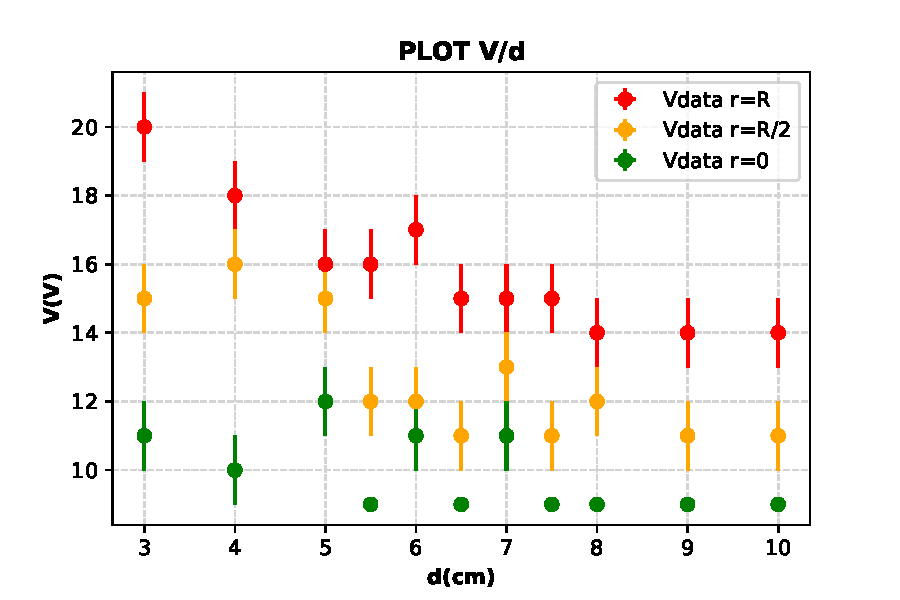
\includegraphics[width=13.5cm]{Figures/Grafico_Parte3_totale.pdf}
  \caption{Grafico della tensione ai capi dell'\emph{ice pail} (in V) in funzione della distanza tra le piastre (in cm). L'errore sulla tensione è pari a $1\%$ del f.s. + $1$ digit, mentre l'errore sulla distanza è di $1 mm$. I tre set corrispondono alle 3 distanze $r$ dal centro dell'armatura dove è stata campionata la carica.}
  \label{fig:GraficoParteIIITotale}
\end{figure}

Il set di dati che più si avvicina all'andamento atteso è quello corrispondente ad $r = R$. I risultati ottenuti sono indicativi del fatto che la carica sulle facce del condensatore aumenta allontanandosi dal centro.

\begin{figure}[H]
  \centering
  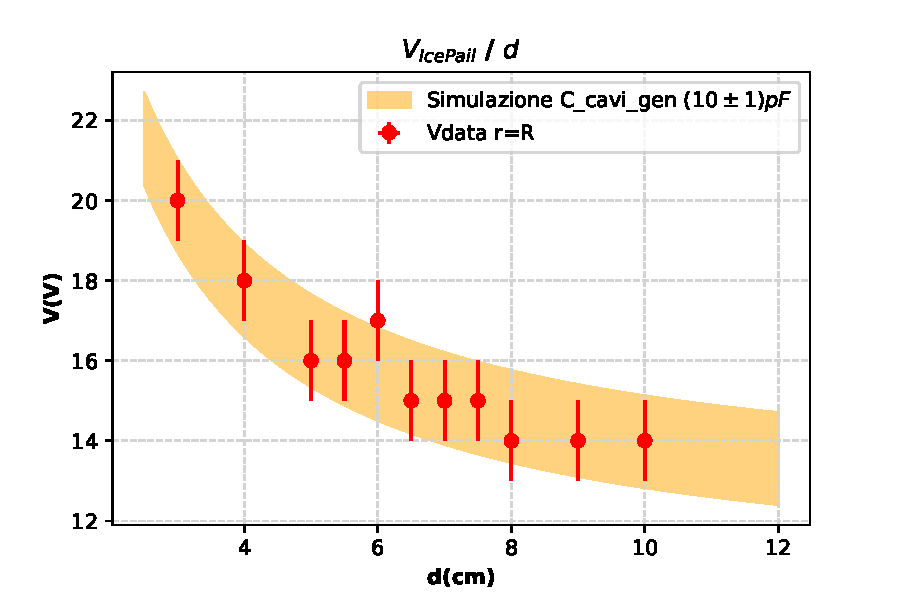
\includegraphics[width=13.5cm]{Figures/Grafico_Parte3.pdf}
  \caption{Grafico della tensione ai capi dell'\emph{ice pail} (in V) in funzione della distanza tra le piastre (in cm). L'errore sulla tensione è pari a $1.3V$, mentre l'errore sulla distanza è di $1 mm$. La simulazione è stata fatta supponendo una capacità dei cavi che collegano il condensatore al generatore di $(10 \pm 1)pF$, considerazione necessaria ai fini della simulazione per poter ricreare l'andamento atteso.}
  \label{fig:GraficoParteIII}
\end{figure}


\par}